%% LyX 2.2.3 created this file.  For more info, see http://www.lyx.org/.
%% Do not edit unless you really know what you are doing.
\documentclass[english]{article}
\usepackage[T1]{fontenc}
\usepackage[latin9]{inputenc}
\usepackage{geometry}
\geometry{verbose,tmargin=2cm,bmargin=2cm,lmargin=2cm,rmargin=2cm,headheight=2cm,headsep=2cm}
\setlength{\parindent}{0bp}
\usepackage{float}
\usepackage{graphicx}

\makeatletter

%%%%%%%%%%%%%%%%%%%%%%%%%%%%%% LyX specific LaTeX commands.
%% Because html converters don't know tabularnewline
\providecommand{\tabularnewline}{\\}

\makeatother

\usepackage{babel}
\begin{document}

\section{Exercise 3}

For this exercise we were asked to implement the Moore machine shown
on Figure \ref{3_1}, but with one condition, everything inside our
machine should work on 3.3v and inputs and outputs should work on
5v logic.

\begin{figure}[H]
\begin{centering}
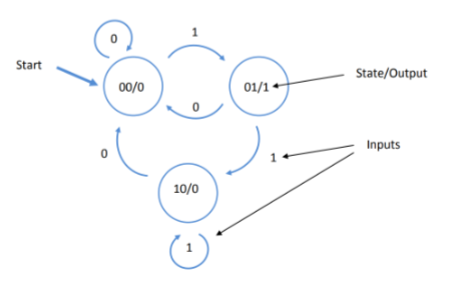
\includegraphics[scale=0.7]{images/Diagram}
\par\end{centering}
\caption{Moore Machine}
\label{3_1}
\end{figure}

\subsection{State Machine Implementation}

We proceeded to convert the diagram to a table that represents it,
and we got Table \ref{3_t_1}, and by transforming each bit (Output,
and next states bits) into a truth table, we could create our logic
implementation for each bit. The Truth Tables are shown on Tables
\ref{3_t_2}.

\begin{table}[H]
\begin{centering}
\begin{tabular}{|c|c|c|c|}
\hline 
State & W=0 & W=1 & Output\tabularnewline
\hline 
\hline 
00 & 00 & 01 & 0\tabularnewline
\hline 
01 & 00 & 10 & 1\tabularnewline
\hline 
10 & 00 & 10 & 0\tabularnewline
\hline 
\end{tabular}
\par\end{centering}
\caption{Moore Machine Table}
\label{3_t_1}

\end{table}

\begin{table}[H]
\begin{centering}
\begin{tabular}{|c|c|}
\hline 
S1 S0 & Output\tabularnewline
\hline 
\hline 
00 & 0\tabularnewline
\hline 
01 & 1\tabularnewline
\hline 
10 & 0\tabularnewline
\hline 
11 & x\tabularnewline
\hline 
\end{tabular} ~%
\begin{tabular}{|c|c|c|c|c|}
\hline 
S1 & S0 & W & S1' & S0'\tabularnewline
\hline 
\hline 
0 & 0 & 0 & 0 & 0\tabularnewline
\hline 
0 & 0 & 1 & 0 & 1\tabularnewline
\hline 
0 & 1 & 0 & 0 & 0\tabularnewline
\hline 
0 & 1 & 1 & 1 & 0\tabularnewline
\hline 
1 & 0 & 0 & 0 & 0\tabularnewline
\hline 
1 & 0 & 1 & 1 & 0\tabularnewline
\hline 
1 & 1 & 0 & x & x\tabularnewline
\hline 
1 & 1 & 1 & x & x\tabularnewline
\hline 
\end{tabular}
\par\end{centering}
\caption{Truth Tables}
\label{3_t_2}

\end{table}

So by re-writing those truth tables we have got the following equations:

\[
Output=S_{1}\,.\,\bar{S_{0}}
\]

\[
S_{1}^{'}=\bar{S_{1}}S_{0}w+S_{1}\bar{S_{0}}w
\]

\[
S_{0}^{'}=\bar{S_{1}}\bar{S_{0}}w
\]

So, by implementing those formulas into a synchronized logic circuit,
we have got the Moore machine.

\subsection{Level Converter Implementation}

To convert the voltage levels on the PCB for compatibility, we decided
to use a 74LS05 Integrated Circuit. It is a inverter with Open-Collector
outputs, that has a $V_{IH_{min}}=2(V)$, which is ideal for our implementation.
By connecting the output to a pull-up network with the voltage we
want, we can convert the level with no problems.

For the Pull-Up network, we decided to use a resistor $R=10\,(k\Omega)$
so that when it's conected to ground, te current flowing through the
inverter is less than $10\,(mA)$, and when the inverter produces
a High Z, the resistor its not enough big to produce a High Z to the
output, and set the output to a logic 1.

\subsection{PCB Implementation}

We proceeded to implement the PCB using Altium Designer, the Schematic
for this Finite State Machine is shown on Figure \ref{3_2}. The Top
and Bottom Layers are shown on Figure \ref{3_3}.

\begin{figure}[H]
\begin{centering}
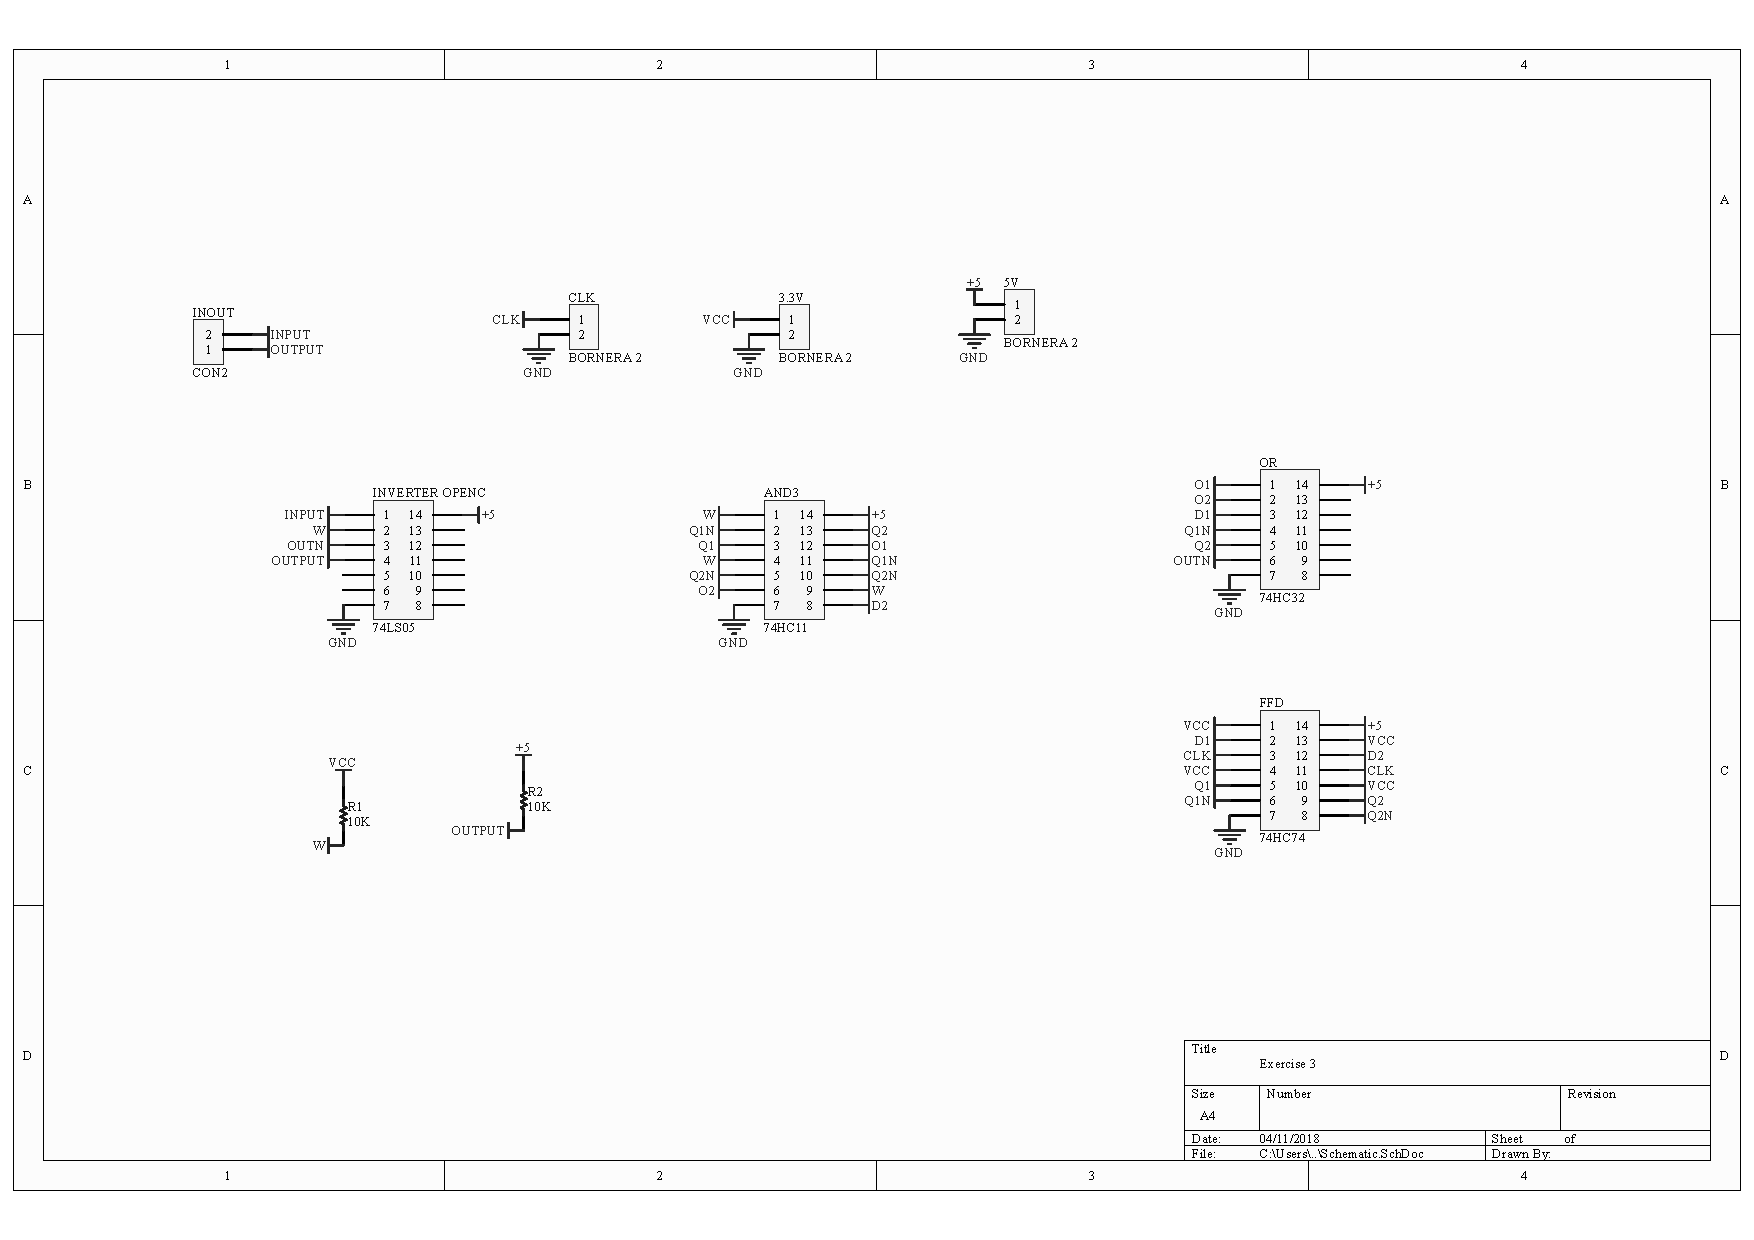
\includegraphics[scale=0.5]{images/Schematic}
\par\end{centering}
\caption{Schematic}
\label{3_2}

\end{figure}

\begin{figure}[H]
\begin{centering}
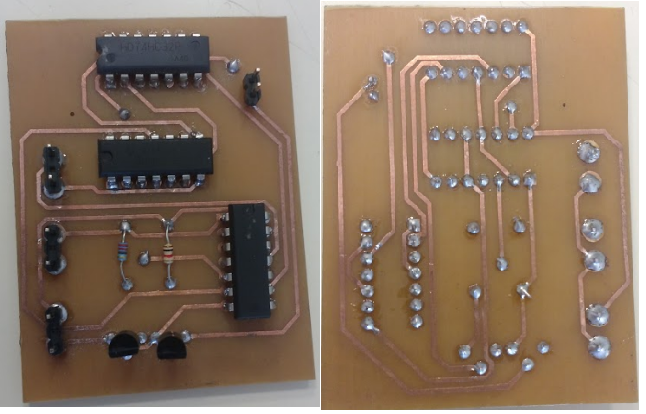
\includegraphics[scale=0.7]{images/TB}
\par\end{centering}
\caption{Top and Bottom Layers}
\label{3_3}

\end{figure}

\end{document}
